\subsection{Generalizirani ICP algoritam}

\subsubsection{Opis algoritma}
Ovaj način uspoređivanja skupova točaka je najjednostavniji. Ne tražimo prepoznatljive oblike niti imamo ikakve posebne optimizacije. Kao ulaz koristimo niz .ply datoteka. Svaka ta dototeka predstavlja jedan skup točaka tj. jedno očitanje lidar-a. Oblik datoteke je prikazan na slici \ref{files:ply_format}. Program otvari dvije datoteke koje predstavljaju dva sljedna očitanja. Tada njihov sadržaj preda metodi koja vraća transformacijsku matricu i fitnes veličinu. Za rad s datotekama se koristi Boost biblioteka otvorenoga koda.


\subsubsection{Izvorni kod algoritma}
Metodom \mintinline{text}{process_files} u primjeru \ref{coderef:gen_icp_process_load} se iterira kroz datoteke te se otvaraju u parovima i njihov sadržaj tj. informacije o oblaku točaka se spremaju u globalne varijable \mintinline{text}{cloud_ref} i \mintinline{text}{cloud_target}. Na linijama 11 i 12 postavljam ICP algoritmu dodatne ulazne parametre, a to su te varijable. Konačno se pokreće algoritam te se ispituje ako je došlo do konvergencije. Do konvergencije dolazi ako su dva skupa oblaka slična tj. ako predstavljaju isti objekt ali rotiran i/ili translantiran. Očekuje se da uvijek dođe do konvergencije u ovome primjeru. Ako je došlo do konvergencije, spremamo podatke u datoteku. Naposljetku se iz optimizacijskih razloga vrijednost matrice \mintinline{text}{cloud_target} sprema kao referentni skup točaka.
\begin{listing}[H]
  \begin{minted}[frame=lines, linenos]{text}
void load_point_cloud(string path, PointCloudType& cloud) {
 pcl::io::loadPLYFile(path, cloud);
}

void process_files(vector<path> paths, ICP icp) {
 for (int i = 0; i < paths.size() - 1; i++) {
  if (i == 0) {
   load_point_cloud(paths.at(i).string(), *cloud_ref);
  }
  load_point_cloud(paths.at(i + 1).string(), *cloud_target);

  string first = paths.at(i).stem().string();
  string second = paths.at(i + 1).stem().string();

  icp.setInputCloud(cloud_ref);
  icp.setInputTarget(cloud_target);
  icp.align(*cloud_reg);

  if (icp.hasConverged()) {
   save_matrix(icp, first, second);
  }
  *cloud_ref = *cloud_target;
 }
}
  \end{minted}
  \caption{Generalizirani ICP - obrada datoteka}
  \label{coderef:gen_icp_process_load}
\end{listing}

\subsubsection{Rezultat algoritma}

\begin{listing}[H]
  \begin{minted}[frame=lines, linenos]{text}
void save_matrix(ICP icp, string first, string second) {
 Matrix4d transformation = icp.getFinalTransformation();
 double fitness = icp.getFitnessScore();
 string filename = first + "-" + second + ".txt";
 Matrix3d mat = mat4x4_to_3x3(transformation);
 Vector3d rpy = mat.eulerAngles(0, 1, 2);
 save_to_file(
   filename,
   mat_to_string(transformation),
   fitness,
   rpy
  );
}
  \end{minted}
  \caption{Generalizirani ICP - spremanje rezultata}
  \label{coderef:gen_icp_save_matrix}
\end{listing}

Spremanje rezultata se vrši metodom \mintinline{text}{save_matrix} u primjeru \ref{coderef:gen_icp_save_matrix}. Matricu transformacije možemo dobiti pozivom \mintinline{text}{icp.getFinalTransformation()} te je  oblika \mintinline{text}{Matrix4d} tj. ima 4 redaka i 4 stupaca dok su elemnti tipa \mintinline{text}{double}. Ta matrica se tada transformira u matricu veličine 3x3 tj. izdvaja se rotacijska matrica zato što takav tip matrice ima ugrađenu metodu \mintinline{text}{eulerAngles()}. Ta metoda kao argumente prima redosljed rotacija objekta tj. redosljed osi rotacija. U ovome slučaju se prvo predaje 0 što znači da se objekt prvo rotirao oko x osi, tada se predaje što znači da se tada rotirao oko y osi i naposljetku se predaje 2 što znači da je zadnja rotacija bila oko z osi. Metoda vraća vektor od tri elementa koji predstavljaju valjanje, poniranje i skretanje. Konačno se sve te informacije spremaju u datoteku s imenom sastavljenim od dva indetifikatora očitanja tako da se zna koji skupovi točaka su upoređivani. Struktura te datoteke je prikazana na primjeru  \ref{files:icp_file_result}. Prva linija sadrži fitnes vrijednost. Od druge do pete linije se nalazi transformacijska matrica dok se na zadnjoj liniji nalaze Eulerovi kutevi u radijanima.
\begin{listing}[H]
  \begin{minted}[frame=lines]{text}
0.0263544
    0.999735   -0.0230172  -0.00046344  -0.00394583
   0.0230173     0.999735  0.000237121  0.000806379
 0.000457859 -0.000247725            1    0.0091155
           0            0            0            1
3.14136 -3.14113 -3.11857
  \end{minted}
  \caption{ICP - datoteka s rezultatom}
  \label{files:icp_file_result}
\end{listing}

\begin{equation}
  \begin{aligned}
AM_{x} &= \frac{1}{n}\sum_{i=0}^{n-1} |X_{i} - \hat{X}_{i}|\\
AM_{y} &= \frac{1}{n}\sum_{i=0}^{n-1} |Y_{i} - \hat{Y}_{i}|\\
AM_{z} &= \frac{1}{n}\sum_{i=0}^{n-1} |Z_{i} - \hat{Z}_{i}|
  \end{aligned}
  \label{eq:coord_am}
\end{equation}
\begin{equation}
  \begin{aligned}
MSE_{x} &= \frac{1}{n}\sum_{i=0}^{n-1} |X_{i} - \hat{X}_{i}|^2\\
MSE_{y} &= \frac{1}{n}\sum_{i=0}^{n-1} |Y_{i} - \hat{Y}_{i}|^2\\
MSE_{z} &= \frac{1}{n}\sum_{i=0}^{n-1} |Z_{i} - \hat{Z}_{i}|^2
  \end{aligned}
  \label{eq:coord_mse}
\end{equation}

\begin{equation}
  \begin{aligned}
ROT_{r} &= \frac{1}{n}\sum_{i=0}^{n-1} |R_{i} - \hat{R}_{i}|\\
ROT_{p} &= \frac{1}{n}\sum_{i=0}^{n-1} |P_{i} - \hat{P}_{i}|\\
ROT_{y} &= \frac{1}{n}\sum_{i=0}^{n-1} |Y_{i} - \hat{Y}_{i}|
  \end{aligned}
  \label{eq:rot_am}
\end{equation}
\begin{equation}
  \begin{aligned}
ROT_{r} &= \frac{1}{n}\sum_{i=0}^{n-1} |R_{i} - \hat{R}_{i}|^2\\
ROT_{p} &= \frac{1}{n}\sum_{i=0}^{n-1} |P_{i} - \hat{P}_{i}|^2\\
ROT_{y} &= \frac{1}{n}\sum_{i=0}^{n-1} |Y_{i} - \hat{Y}_{i}|^2
  \end{aligned}
  \label{eq:rot_mse}
\end{equation}

Sretnja aritmetička vrijednosti apsolutnih razlika koordinata i rotacija se računa s formulama \ref{eq:coord_am} i \ref{eq:rot_am}. Element $n$ je ukupan broj točaka, $X_{i}$ je stvarna vrijednost koordinate x, dok je $\hat{X}_{i}$ estimirani iznos x koordinate. Element $R_{i}$ je stvarna vrijednost kura valjanja, dok je $\hat{R}_{}$ estimirana vrijednost kuta valjanja. Srednje vrijednosti kvadrata razlika za koordinate i rotacije se računaju s formulama \ref{eq:coord_mse} i \ref{eq:rot_mse}. Rezultati su prikazani u tablici \ref{res:ref_est_table}. AM znači aritmetička sredina, dok MSE znači aritmetička sredina kvadrata razlike.

\begin{table}[H]
  \centering
  \begin{tabular}{ |p{3cm}| |p{3cm}|p{3cm}| }
    \hline
    Rezultati& Primjer A& PrimjerB\\
    \hline
    Duljina [m]& 677.521& 467.367\\
    AMx [m]& 1.861& 0.927\\
    AMy [m]& 2.543& 1.019\\
    AMz [m]& 0.084& 0.016\\
    AMr [rad]& 9.887E-4& 2.813E-4\\
    AMp [rad]& 9.356E-4& 3.680E-4\\
    AMy [rad]& 0.351& 0.012\\
    \hline
    MSEx [$m^2$]& 7.301& 1.953\\
    MSEy [$m^2$]& 8.268& 1.442\\
    MSEz [$m^2$]& 0.015& 5.642E-4\\
    MSEr [$rad^2$]& 9.229-6& 1.903E-6\\
    MSEp [$rad^2$]& 4.331-6& 6.047E-7\\
    MSEy [$rad^2$]& 1.981& 2.622E-4\\
    \hline
  \end{tabular}
  \caption{Usporedbe referentnih i estimiranih podataka}
  \label{res:ref_est_table}
\end{table}
\pagebreak

\subsubsection{Evaluacija rezultata za primjer A}
\begin{figure}[H]
  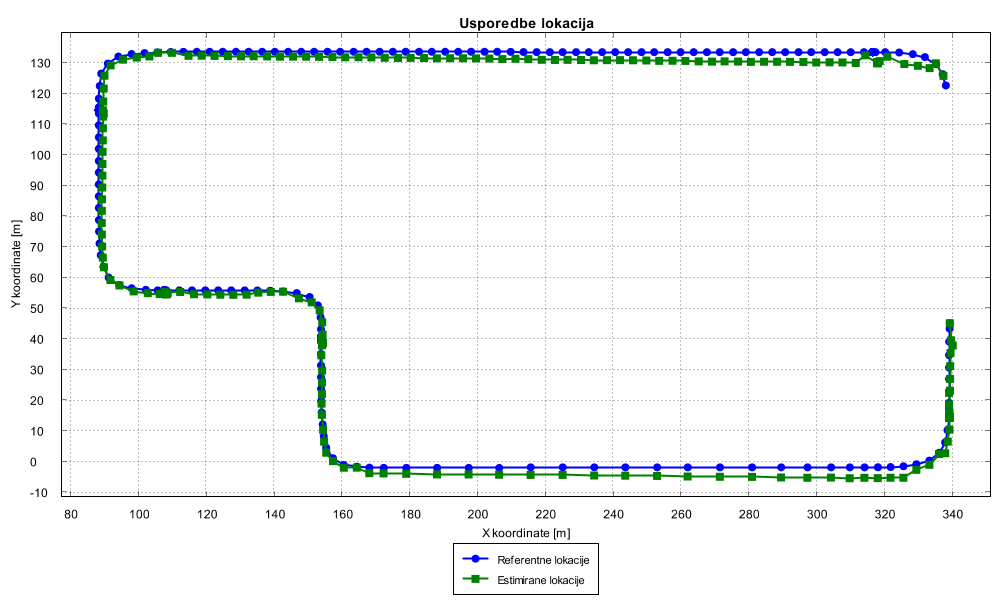
\includegraphics[scale=0.4]{images/algo1/primjer3/usporedba_lokacija.png}
  \caption{Graf lokacije vozila}
  \label{eval:a1p3_lokacija}
\end{figure}
\begin{figure}[H]
  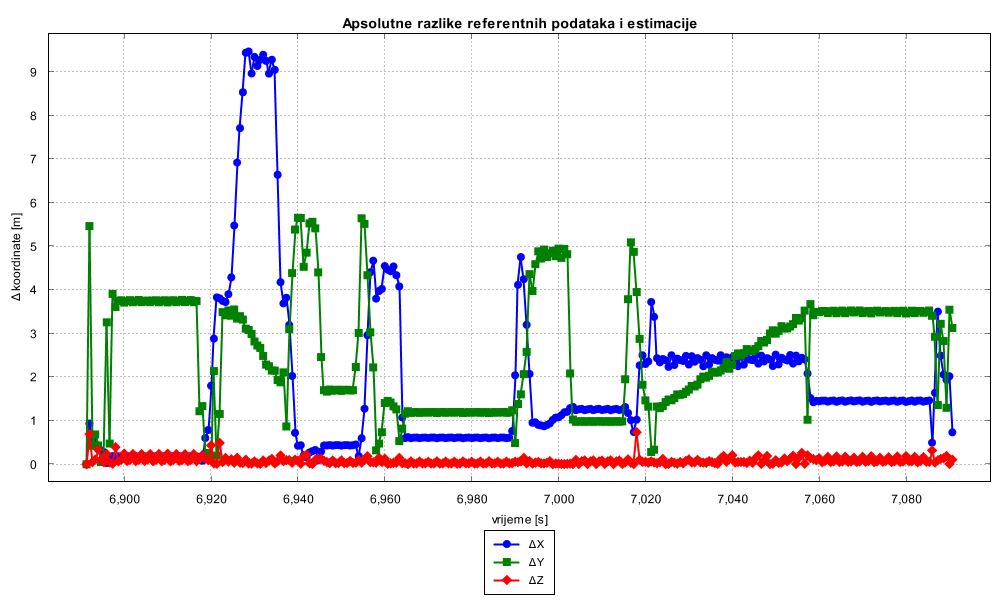
\includegraphics[scale=0.4]{images/algo1/primjer3/apsolutne_razlike_koordinata.png}
  \caption{Apsolutne razlike koordinata}
  \label{eval:a1p3_koord_razlike}
\end{figure}
\begin{figure}[H]
  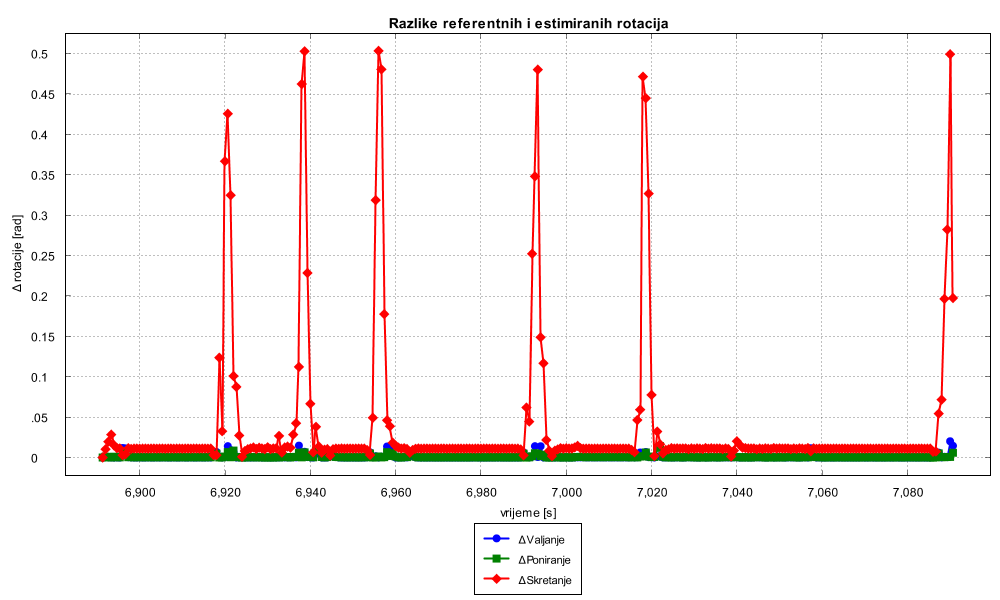
\includegraphics[scale=0.4]{images/algo1/primjer3/rotacije_razlike.png}
  \caption{Apsolutne razlike rotacija}
  \label{eval:a1p3_rot_razlike}
\end{figure}
\begin{figure}[H]
  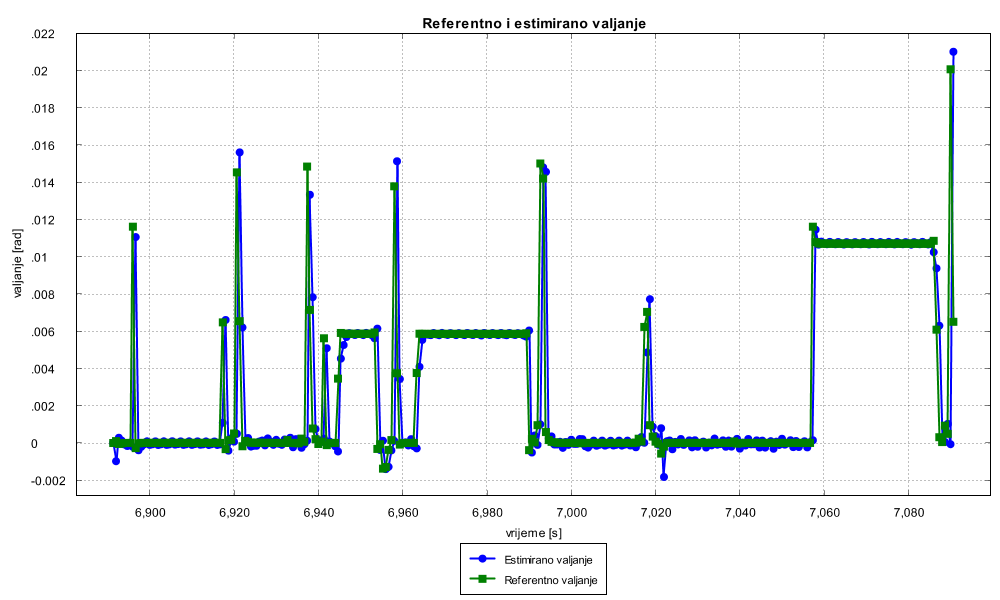
\includegraphics[scale=0.4]{images/algo1/primjer3/referentno_estimirano_valjanje.png}
  \caption{Usporedba referentnog i estimiranog valjanja}
  \label{eval:a1p3_rot_roll}
\end{figure}
\begin{figure}[H]
  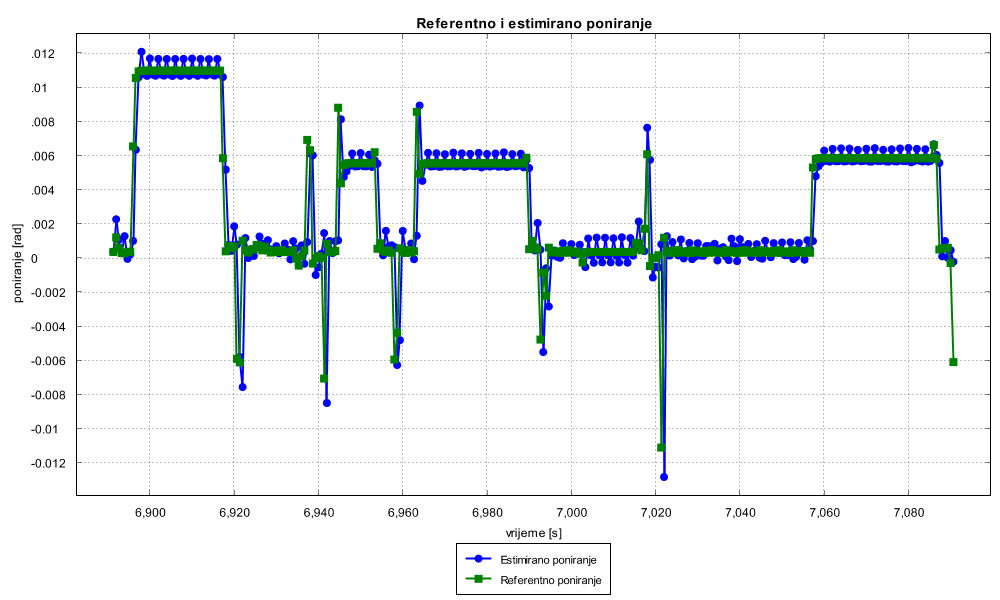
\includegraphics[scale=0.4]{images/algo1/primjer3/referentno_estimirano_poniranje.png}
  \caption{Usporedba referentnog i estimiranog poniranja}
  \label{eval:a1p3_rot_pitch}
\end{figure}
\begin{figure}[H]
  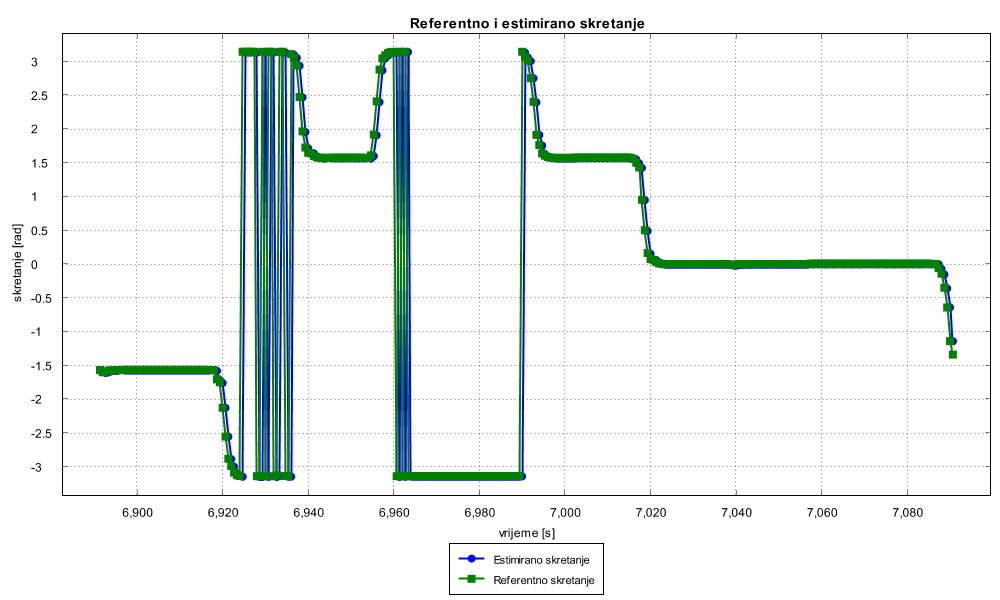
\includegraphics[scale=0.4]{images/algo1/primjer3/referentno_estimirano_skretanje.png}
  \caption{Usporedba referentnog i estimiranog skretanja}
  \label{eval:a1p3_rot_yaw}
\end{figure}


\subsubsection{Evaluacija rezultata za primjer B}
\begin{figure}[H]
  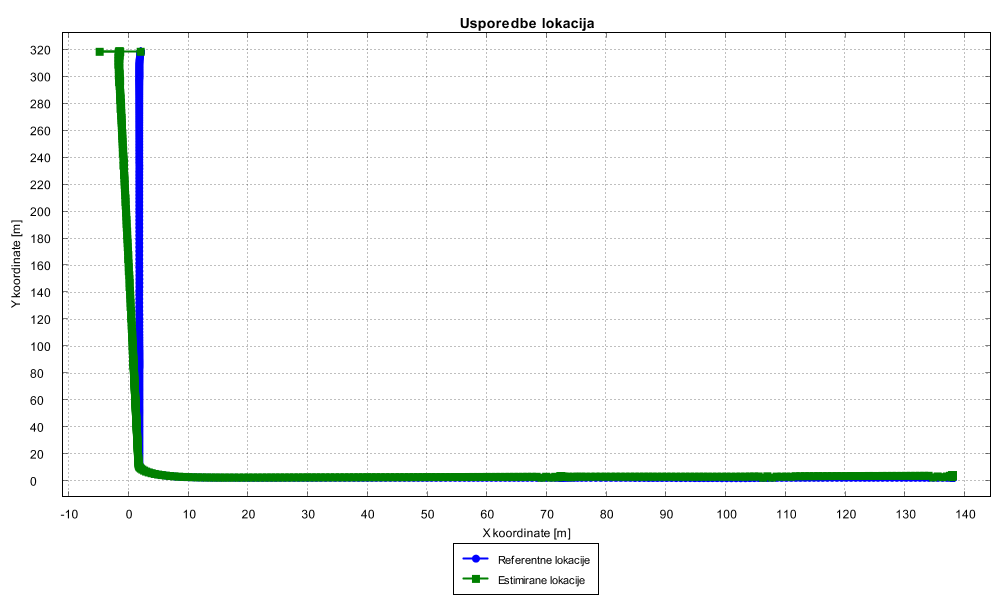
\includegraphics[scale=0.4]{images/algo1/primjer4/usporedba_lokacija.png}
  \caption{Graf lokacije vozila}
  \label{eval:a1p4_lokacija}
\end{figure}
\begin{figure}[H]
  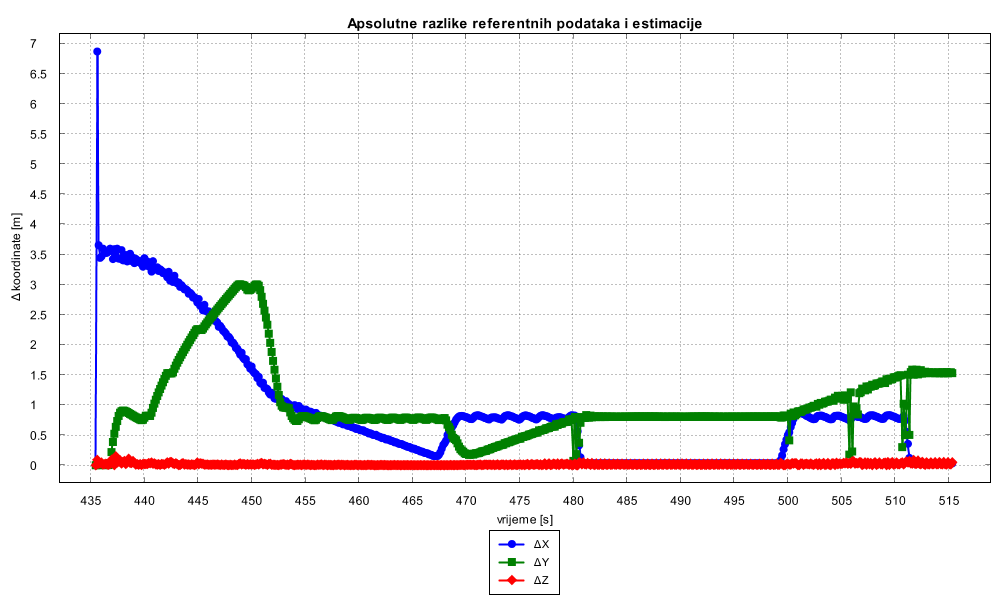
\includegraphics[scale=0.4]{images/algo1/primjer4/apsolutne_razlike_koordinata.png}
  \caption{Apsolutne razlike koordinata}
  \label{eval:a1p4_koord_razlike}
\end{figure}
\begin{figure}[H]
  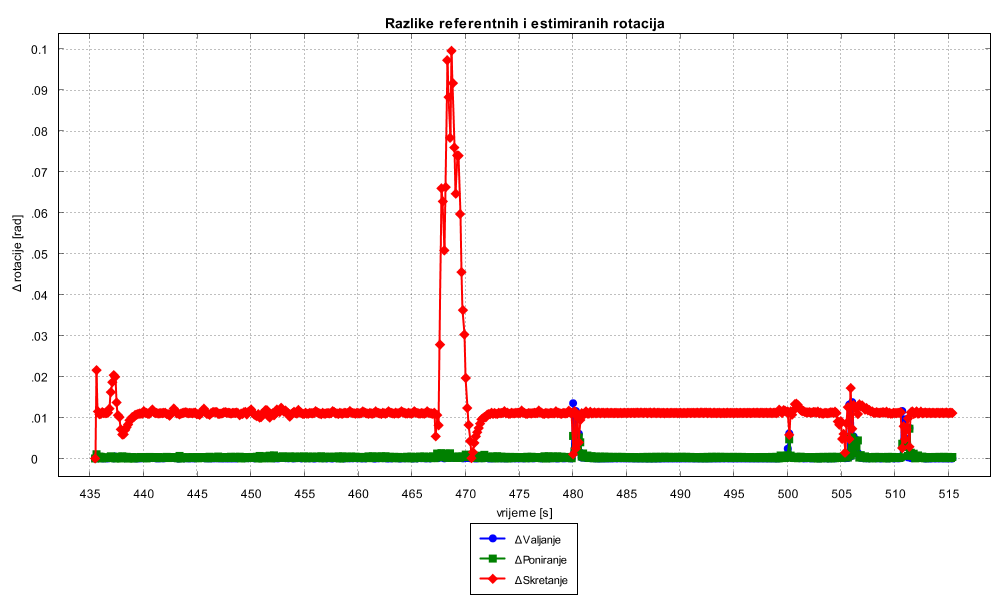
\includegraphics[scale=0.4]{images/algo1/primjer4/rotacije_razlike.png}
  \caption{Apsolutne razlike rotacija}
  \label{eval:a1p4_rot_razlike}
\end{figure}
\begin{figure}[H]
  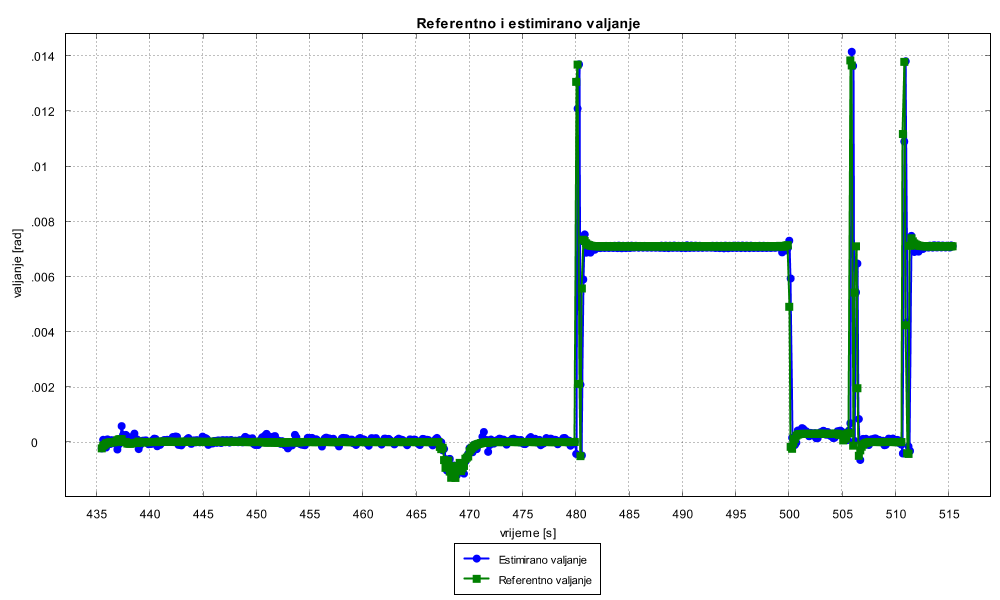
\includegraphics[scale=0.4]{images/algo1/primjer4/referentno_estimirano_valjanje.png}
  \caption{Usporedba referentnog i estimiranog valjanja}
  \label{eval:a1p4_rot_roll}
\end{figure}
\begin{figure}[H]
  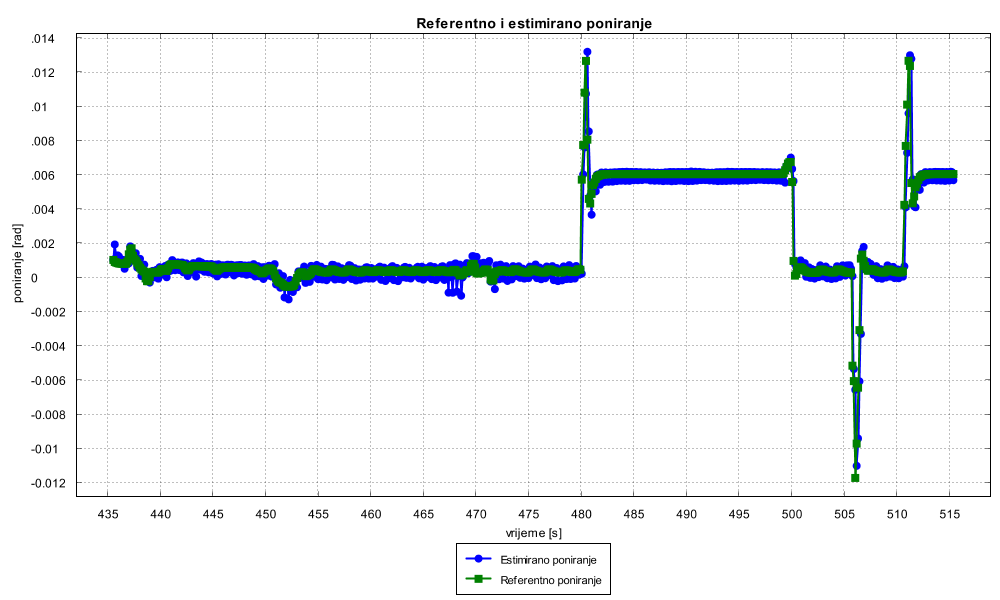
\includegraphics[scale=0.4]{images/algo1/primjer4/referentno_estimirano_poniranje.png}
  \caption{Usporedba referentnog i estimiranog poniranja}
  \label{eval:a1p4_rot_pitch}
\end{figure}
\begin{figure}[H]
  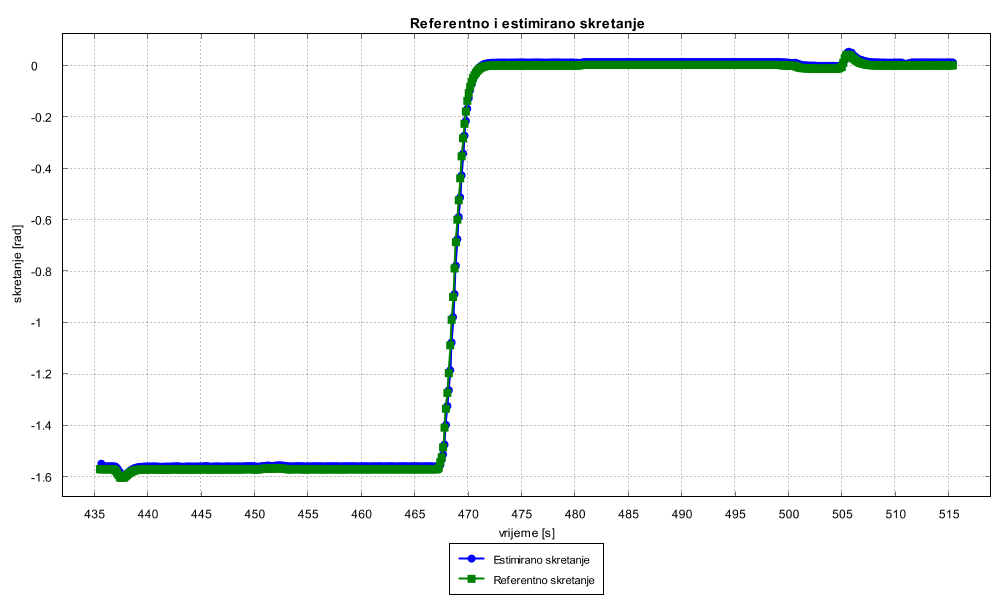
\includegraphics[scale=0.4]{images/algo1/primjer4/referentno_estimirano_skretanje.png}
  \caption{Usporedba referentnog i estimiranog skretanja}
  \label{eval:a1p4_rot_yaw}
\end{figure}
\pagebreak